\documentclass{article}
\usepackage{tikz, comment}
\usepackage{pifont}
\usepackage{fontspec, pgfplots}
\usetikzlibrary{arrows, decorations.markings, decorations.pathreplacing}
\begin{comment}
:Title: Not defined yet
:Tags: perimeter;origin;end behavior;pappus&#146;s theorem, theorem of pappus;median of a trapezoid
:Prob: 0.6357;0.6027;0.598;0.5951;0.5846
:Author: Prof.Hu Ji-shan, HKUST
:Slug: No name yet

Description Here.........
\end{comment}
\begin{document}\centering 

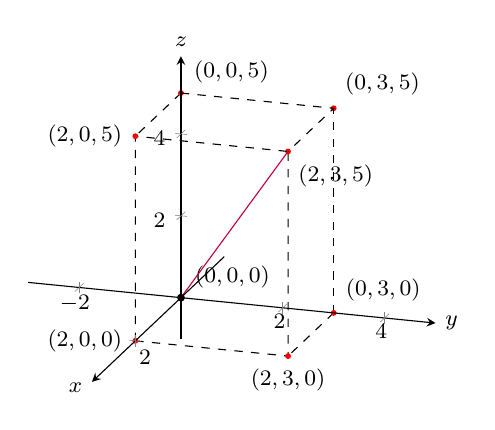
\begin{tikzpicture}[font=\footnotesize]
\pgfplotsset{compat=1.8}
\begin{axis}
[axis lines = center, view={108}{25},
axis on top, xlabel = {$x$}, ylabel ={$y$}, zlabel ={$z$}, domain =0:1, y domain =0:1,
xmin =-1.9,
xmax =3.9,
ymin =-3.0,
ymax =5,
zmin =-1.0, 
zmax =5.9,
samples =10, samples y =40, z buffer =sort, 
every axis x label/.style={
    at={(ticklabel* cs:1)},
    anchor= east, yshift =-2
},
every axis y label/.style={
    at={(ticklabel* cs:1)},
    anchor= west,
},
every axis z label/.style={
    at={(ticklabel* cs:1)},
    anchor= south
},]

\addplot3[dashed] coordinates
        {(2,3,5) (2,3,0) (2,0,0)};
\node[label={-80:{$(2,3,5)$}},circle,fill=red,inner sep=0.75pt] at (axis cs:2,3,5) {};
\node[label={180:{$(2,0,0)$}},circle,fill=red,inner sep=0.75pt] at (axis cs:2,0,0) {};
\node[label={-90:{$(2,3,0)$}},circle,fill=red,inner sep=0.75pt] at (axis cs:2,3,0) {};
\addplot3[dashed] coordinates
        {(2,3,0) (0,3,0)};

\addplot3[dashed] coordinates
        {(2,0,0) (2,0,5) (2,3,5)};
\node[label={180:{$(2,0,5)$}},circle,fill=red,inner sep=0.75pt] at (axis cs:2,0,5) {};

\addplot3[dashed] coordinates
        {(2,0,5) (0,0,5)};
\node[label={10:{$(0,0,5)$}},circle,fill=red,inner sep=0.75pt] at (axis cs:0,0,5) {};
\node[label={60:{$(0,3,5)$}},circle,fill=red,inner sep=0.75pt] at (axis cs:0,3,5) {};
\addplot3[dashed] coordinates
		{(0,3,5) (0,0,5) (2,3,5)};

\addplot3[dashed] coordinates
        {(0,3,5) (0,3,0)};
\node[label={45:{$(0,3,0)$}},circle,fill=red,inner sep=0.75pt] at (axis cs:0,3,0) {};

\node[label={3:{$(0,0,0)$}},circle,fill, inner sep=1pt] at (axis cs:0,0,0) {};

\addplot3[purple] coordinates
        {(0,0,0) (2,3,5)};
        
\end{axis}

\end{tikzpicture}
\end{document}